\textbf{10-1.}人耳能听到的声音频率范围一般为 $20 \sim 20000 \mathrm{~Hz}$ 。试计算在 $25^{\circ} \mathrm{C}$ 的海水中人耳能听到的声音的波长范围。已知声音在 $25^{\circ} \mathrm{C}$ 海水中的传播速度为 $1531 \mathrm{~m} / \mathrm{s}$ 。

\vfill

\textbf{10-2.}由海底的地震所激发的潮浪, 称为海啸。由于大洋的平均深度大约是 $5 \mathrm{~km}$ , 而潮浪的水平长度大于 $5 \mathrm{~km}$ , 故可认为是一种浅水波。若海底地震的震中与海岸的距离为 $100 \mathrm{~km}$ , 试估算潮浪传到海岸所需的时间。

\vfill
\newpage

\textbf{10-3.}设有一简谐横波 $y = 5.0 \cos \left[2\pi \left(\frac{t}{0.05} - \frac{x}{10}\right)\right]$ ，其中 $x, y$ 的单位为 $\mathrm{cm}, t$ 的单位为 $\mathbf{s}$ 。试求：

(1) 振幅 A、频率 v、波长 $\lambda$ 以及波速 v；

(2) 若某处振动的初相位为 $\frac{3}{5}\pi$ ，求该处的位置 x。

\vfill

\textbf{10-4.}一根质量线密度为 $4 \times 10^{-3} \mathrm{~kg} / \mathrm{m}$ 的均匀钢丝, 被 $10 \mathrm{~N}$ 的力所拉紧。钢丝的一端有一正弦式的横向波扰动, 经过 $0.1 \mathrm{~s}$ , 此波扰动即传到钢丝的另一端, 而扰动源正好经历 100 个周期。求波长。

\vfill
\newpage

\textbf{10-5.}一正弦横波沿一弦线自左向右传播,传播速度为 $80 \mathrm{~cm} / \mathrm{s}$ 。观察弦上某点的运动,发现该点在做振幅为 $2 \mathrm{~cm}$ 、频率为 $10 \mathrm{~Hz}$ 的简谐振动。若取该点为坐标 $x$ 的原点,当 $t = 0$ 时,该点正好位于原点,且具有向 $y$ 轴正方向运动的速度。试求:

(1) 此波的波长 $\lambda$ ;

(2) 弦上该点的振动方程;

(3) 此波的运动学方程;

(4) 弦上 $x = 4 \mathrm{~cm}$ 处质点振动的初相位 $\varphi'$ 。

\vfill

\textbf{10-6.}设入射波的方程为 $y = 0.2\cos (\pi t - 1.5\pi x + 0.4\pi)$ ，其中 $x, y$ 的单位是 $m, t$ 的单位是 $s$ 。波在 $x = 0$ 处反射。试就以下两种情况，求在振幅不衰减情况下合成驻波的方程，并指出 $x = 0$ 处是波节还是波腹。

(1) x=0 处是自由端；

(2) x=0 处是固定端。

\vfill
\newpage

\textbf{10-7.}两根完全相同的琴弦, 它们的基频都是 $357 \mathrm{~Hz}$ 。其中一根琴弦的弦轴略有松动, 以致该弦的张力以恒定的速率减小, 其每秒减小量 $\Delta F_{\mathrm{T}}$ 与原张力 $F_{\mathrm{T} 0}$ 之比为 0.001 。问经过多少时间, 此两琴弦同时发声时会产生 $1 \mathrm{~Hz}$ 的拍频?

\vfill

\textbf{10-8.}一装置于海底的超声波探测器, 发出一束频率为 $30000 \mathrm{~Hz}$ 的超声波, 被向着探测器驶来的潜艇反射回来, 反射波与原来的波合成后, 得到频率为 $241 \mathrm{~Hz}$ 的拍。求潜艇的速率。设超声波在海水中的波速为 $1500 \mathrm{~m} / \mathrm{s}$ 。

\vfill
\newpage

\textbf{10-9.}一平面简谐波沿 $x$ 轴方向传播, 其表示式为
$$
y = A \cos (\omega t - k x + \varphi_ {0})
$$
在 $x=x_{0}$ 固定端处反射。求反射波的表示式，振幅不衰减。

\vfill

\textbf{10-10.}在绳索上传播的波, 其表示式为 $y = 3\cos \left[2\pi \left(\frac{t}{0.1} - \frac{x}{10}\right) - \frac{\pi}{3}\right]$ , 式中 $x, y$ 的单位为 $\mathrm{cm}, t$ 的单位为 $\mathrm{s}$ 。为在绳索上形成驻波 (在 $x = 0$ 处为波节), 则应叠加一个什么样的波? 写出此波的表示式。并写出驻波的表示式。

\vfill
\newpage


\textbf{10-11.}一波沿 $x$ 轴传播, 观察到 $x$ 轴上两点 $x_{1}$ 和 $x_{2}$ 处介质的质点均做频率为 $2.0 \mathrm{~Hz}$ 的简谐振动, $x_{1}$ 处振动相位比 $x_{2}$ 处落后 $\frac{\pi}{4}$ 。已知 $x_{2} - x_{1} = 3.0 \mathrm{~cm}$ 。

(1) 试问此波是沿正 x 轴方向传播, 还是沿负 x 轴方向传播? (设 $\lambda > 6 \, cm$ )

(2) 试求波长 $\lambda$ 和波速 v。

\vfill

\textbf{10-12.}在拉紧的弦上传播的一个波脉冲可表示为
$$
y (x, t) = \frac {b ^ {3}}{b ^ {2} + (2 x - u t) ^ {2}}
$$
式中 b、u 均为常量。

(1) 画出 t=0 时的波形图。

(2) 波脉冲传播的速率及方向如何?

(3) 试求 $t = 0$ 时刻弦上任一点 $x$ 的横向速度。


\vfill
\newpage

\textbf{10-13.}入射波在固定端全反射,某一瞬时的波形如习题 10- 13 图(a)所示。试画出此瞬时反射波的波形图。

\begin{figure}[H]
  \centering
  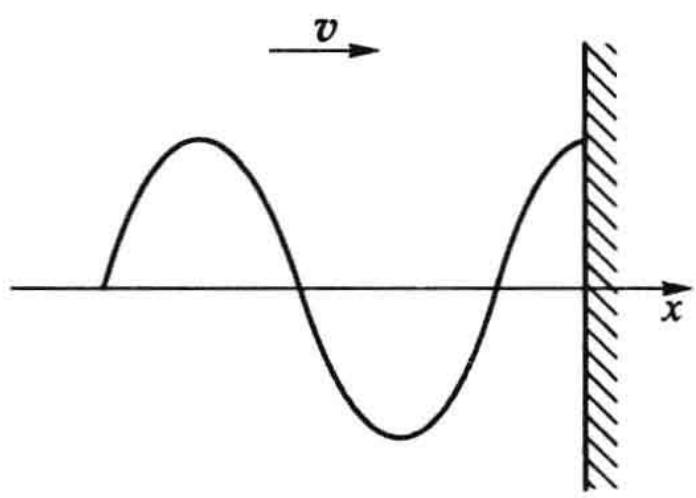
\includegraphics[width=0.3\textwidth]{figures/fig10-13_b.jpg}
  \end{figure}

\vfill

\textbf{10-14.}如习题 10-14 图所示, 一根线密度为 $0.15 \mathrm{~g} / \mathrm{cm}$ 的弦线, 其一端与一频率为 $50 \mathrm{~Hz}$ 的音叉相连, 另一端跨过一定滑轮后悬一重物给弦线提供张力, 重物质量为 $m$ , 音叉到滑轮间的距离为 $1 \mathrm{~m}$ . 当音叉振动时, 为使弦上形成一个、两个、三个波腹, 则重物的质量 $m$ 应各为多大?

\begin{figure}[H]
  \centering
  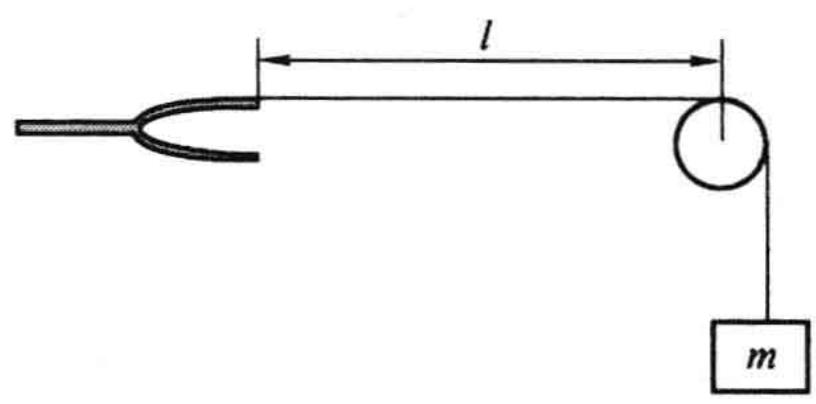
\includegraphics[width=0.35\textwidth]{figures/fig10-14.jpg}
  \end{figure}

\vfill
\newpage

\textbf{10-15.}在一半径为 $10 \mathrm{~cm}$ 的圆柱形管子里, 一平面简谐空气波沿轴向传播, 波长和频率分别为 $\lambda = 80 \mathrm{~cm}, \nu = 425 \mathrm{~Hz}$ , 波的能流密度为 $1.7 \times 10^{-2} \mathrm{~J} / (\mathrm{~s} \cdot \mathrm{m}^{2})$ 。试求:

(1) 管中波的平均能量密度和最大能量密度;

(2) 每两个相邻同相位面间的总能量。

\vfill

\textbf{10-16.}一波源以 $35000 \mathrm{~W}$ 的功率发射球面电磁波。在某处测得该波的平均能量密度为 $7.8 \times 10^{-15} \mathrm{~J} / \mathrm{m}^{3}$ 。求该处离波源的距离。电磁波的传播速度为 $3.0 \times 10^{8} \mathrm{~m} / \mathrm{s}$ 。

\vfill
\newpage

\textbf{10-17.}以下两列波在介质中叠加：
$$
y _ {1} = A \cos (6 t - 5 x), y _ {2} = A \cos (5 t - 4 x)
$$
(式中 $x, y_{1}, y_{2}$ 的单位是 m, t 的单位是 s)

(1) 求此两列波的相速度 $v_{p1}$ 、 $v_{p2}$ ;

(2) 写出合成波的方程, 并求出振幅为零的相邻两点之间的距离;

(3) 求群速度 $v_{g}$ 。

\vfill

\textbf{10-18.}水上短波长 $(\lambda \leqslant 1 \mathrm{~cm})$ 的涟波运动, 是受表面张力控制的。这种涟波的相速度为 $v_{\mathrm{p}} = \left(\frac{2 \pi \sigma}{\rho \lambda}\right)^{\frac{1}{2}}$ , 式中 $\sigma$ 为表面张力系数, $\rho$ 为水的密度。

(1) 证明:由接近某给定波长 $\lambda$ 的诸波长所构成的扰动,群速度等于 $\frac{3}{2}v_{p}$ ;

(2) 若波群只有两个波组成, 此两波的波长分别为 $0.99 \mathrm{~cm}$ 和 $1.01 \mathrm{~cm}$ , 则波群两相邻峰值间的距离为多大?

\vfill
\newpage

\textbf{10-19.}对于深水波,考虑到表面张力,其色散关系为 $\omega^2 = g k + \frac{\sigma k^3}{\rho}$ ,式中水的密度 $\rho = 1.0 \times 10^{3} \mathrm{~kg} / \mathrm{m}^{3}$ , 表面张力 $\sigma = 7.2 \times 10^{-2} \mathrm{~N} / \mathrm{m}$ 。

(1) 求出相速度和群速度与 k 的函数关系;

(2) 证明对于波长接近 $1.7 \times 10^{-2} \mathrm{~m}$ 的诸波所构成的水波, 其相速度与群速度相等, 并求出速度值。

\vfill

\textbf{10-20.}把两根连在一起的弦线拉紧,设想有一行波入射到相接处,为使反射波的振幅 $B$ 与入射波的振幅 $A$ 之比 $\frac{B}{A} = \frac{1}{3}$ 。试求:

(1) 两根弦线的线密度之比 $\eta_{1}: \eta_{2}$ , 设入射波从弦线 1 向弦线 2 方向传播;

(2) 透射波的振幅 C 与入射波振幅 A 之比 $\frac{C}{A}$ 。

\vfill
\newpage

\textbf{10-21.}一列纵波在两种介质的界面上发生反射。设入射波与反射波的振动方向不变, 在入射波所在的介质中纵波的波速是横波波速的 $\sqrt{3}$ 倍。试问为使反射波是一横波, 则入射角应为多大?

\begin{figure}[H]
  \centering
  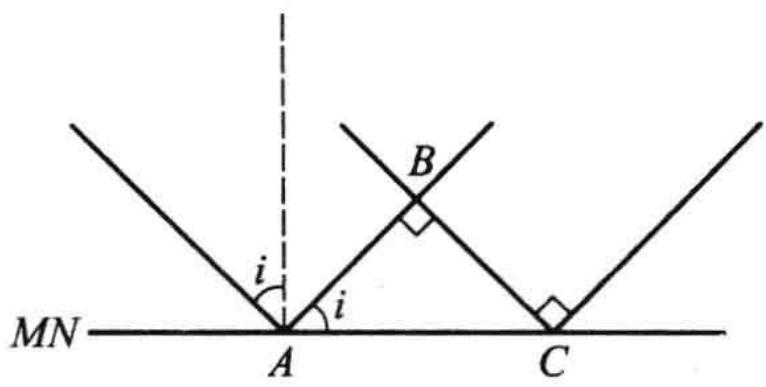
\includegraphics[width=0.4\textwidth]{figures/fig10-21.jpg}
\end{figure}

\vfill
\newpage